\documentclass{article}
\usepackage{amsmath} %This allows me to use the align functionality.
                     %If you find yourself trying to replicate
                     %something you found online, ensure you're
                     %loading the necessary packages!
\usepackage{amsfonts}%Math font
\usepackage{graphicx}%For including graphics
\usepackage{hyperref}%For Hyperlinks
\usepackage{natbib}        %For the bibliography
\bibliographystyle{apalike}%For the bibliography
\usepackage[margin=1.0in]{geometry}
\usepackage{float}
\usepackage{Sweave}
\begin{document}
\Sconcordance{concordance:HW1.tex:HW1.Rnw:%
1 12 1 1 0 14 1 1 3 7 0 1 2 7 0 1 2 44 1 1 4 3 0 1 2 1 0 1 2 1 0 1 1 3 %
0 1 2 27 1 1 3 2 0 2 1 3 0 2 2 1 0 1 5 7 0 1 2 1 1 1 3 12 0 1 9 1 1 1 3 %
8 0 1 5 1 1 1 8 13 0 1 5 1 1 1 3 2 0 2 1 7 0 1 6 1 1 1 3 25 0 1 22 1 1 %
1 4 3 0 2 1 3 0 1 2 1 26 1 2 4 1 1 16 1 2 3 1 1 12 1 2 3 1 1 8 1 2 4 1 %
1 3 2 0 1 10 9 0 1 2 1 10 9 0 1 1 3 0 1 2 1 3 2 0 1 6 5 0 1 1 1 6 5 0 1 %
1 3 0 1 2 1 9 8 0 1 2 1 0 2 2 1 0 1 2 1 3 1 0 1 1 1 9 8 0 1 1 35 0 1 34 %
4 1 1 3 5 0 1 2 22 1 1 3 5 0 1 2 25 1 1 3 2 0 2 1 1 18 22 0 1 5 1 1 1 3 %
2 0 1 1 1 7 5 0 1 7 19 0 1 2 1 1 1 5 4 0 1 6 4 0 1 1 20 0 1 2 1 1 1 2 1 %
0 1 1 3 0 1 2 1 10 1 2 5 1 1 3 2 0 1 11 9 0 1 4 16 0 1 2 1 1 1 5 4 0 1 %
8 6 0 1 5 3 0 1 1 20 0 1 2 1 1 1 4 3 0 1 4 2 0 1 2 1 0 1 1 1 2 1 0 1 1 %
4 0 1 3 1 10 1 2 6 1}

%set the size of the graphs to fit nicely on a 8.5x11 sheet
\noindent \textbf{MA 354: Data Analysis I -- Fall 2019}\\%\\ gives you a new line
\noindent \textbf{Homework 1:}\vspace{1em}\\
\emph{Complete the following opportunities to use what we've talked about in class. 
These questions will be graded for correctness, communication and succinctness. Ensure
you show your work and explain your logic in a legible and refined submission.}\\
%Comments -- anything after % is not put into the PDF

You can complete questions 1-2 now. Split into groups of two and each group
will complete the following to do list -- you can split into groups and
select the question to work on naturally or you can ask \texttt{R} to do 
it for you as follows. (I often use this functionality to choose where to
eat or what movie to watch).
\begin{Schunk}
\begin{Sinput}
> #Denote Group 1
> sample(x = c("Student1","Student2","Student3","Student4"),size=2,replace=F)
\end{Sinput}
\begin{Soutput}
[1] "Student1" "Student2"
\end{Soutput}
\begin{Sinput}
> #Denotes which question group 1 will do
> sample(x=c(1,2),size=1)
\end{Sinput}
\begin{Soutput}
[1] 1
\end{Soutput}
\end{Schunk}

\begin{itemize}
  \item \textbf{Stage 1} each student in the subgroup will provide a solution
  \item \textbf{Stage 2} the subgroup will compare solutions and choose the best aspects
  of each toward having a better, combined solution.
  \item \textbf{Stage 3} each student will read and edit the solution sequentially
  \item \textbf{Stage 4} the subgroups will swap solutions for constructive feedback 
  and suggestions
  \item \textbf{Stage 5} the subgroups will edit their solutions to address all constructive 
  feedback
  \item \textbf{Stage 6} each student will check both solutions for completeness, making
  any necessary adjustments sequentially until both solutions are agreed upon.
\end{itemize}

For subsequent questions, students will do the same thing keeping the same subgroups
or swapping if desired. While students have assigned jobs for specified questions, 
I encourage students to help with all parts of each question in collaboration with 
other students in the group.
\newpage

\begin{enumerate}
%%%%%%%%%%%%%%%%%%%%%%%%%%%%%%%%%%%%%%%%%%%%%%%%%%%%%%%%%%%%%%%%%%%%%%%%%%%%%%%
%%%%%%%%%%%%%%%%%%%%%%%%%%%%%%%%%%%%%%%%%%%%%%%%%%%%%%%%%%%%%%%%%%%%%%%%%%%%%%%
%%%%%%%%%  Question 0
%%%%%%%%%%%%%%%%%%%%%%%%%%%%%%%%%%%%%%%%%%%%%%%%%%%%%%%%%%%%%%%%%%%%%%%%%%%%%%%
%%%%%%%%%%%%%%%%%%%%%%%%%%%%%%%%%%%%%%%%%%%%%%%%%%%%%%%%%%%%%%%%%%%%%%%%%%%%%%%
  \item[0.] \textbf{Complete weekly diagnostics.}
%%%%%%%%%%%%%%%%%%%%%%%%%%%%%%%%%%%%%%%%%%%%%%%%%%%%%%%%%%%%%%%%%%%%%%%%%%%%%%%
%%%%%%%%%%%%%%%%%%%%%%%%%%%%%%%%%%%%%%%%%%%%%%%%%%%%%%%%%%%%%%%%%%%%%%%%%%%%%%%
%%%%%%%%%  Question 1
%%%%%%%%%%%%%%%%%%%%%%%%%%%%%%%%%%%%%%%%%%%%%%%%%%%%%%%%%%%%%%%%%%%%%%%%%%%%%%%
%%%%%%%%%%%%%%%%%%%%%%%%%%%%%%%%%%%%%%%%%%%%%%%%%%%%%%%%%%%%%%%%%%%%%%%%%%%%%%%
\item \textbf{(Data Cleaning and Summary)} In recent work, psychology researchers 
investigated how subjective socioeconomic status affects how participants experience
negative and positive emotions and whether or not the effect is different by race. 

The researchers recruited particpants via Amazon MTurk Prime Panels to complete the 
study. Amazon provides all of the data separated by race, and a separate file denoting 
which observations yield a representative sample based on age, education, and other 
control variables. Below, you will work to combine these datasets into one workable
file you can use to summarize the data.

\begin{enumerate}
\item Load Data. There are over 100 columns, so we don't print previews of the data
like we did previously.
\begin{Schunk}
\begin{Sinput}
> ###Download data
> dat.white<-read.csv("https://cipolli.com/students/data/WhiteParticipants.txt",
+ header=T,sep=",")
> dat.black<-read.csv("https://cipolli.com/students/data/BlackParticipants.txt",
+ header=T,sep=",")
> dat.matched<-read.csv("https://cipolli.com/students/data/matchedsample.txt",
+ header=T,sep=",")
> colnames(dat.matched)<-c("aid","id","MatchedSample")
\end{Sinput}
\end{Schunk}
\item Remove non-white observations from \texttt{dat.white}; i.e., remove observations 
from \texttt{dat.white} where Race does not equal 1.
\item Create an object called \texttt{dat.wb} that contains all of the observations;
i.e., merge the data loaded from WhiteParticipants.csv and BlackParticipants.csv.
\item The aid of observations that make up a representative sample have a value of
1; i.e., observation $i$ is in the representative sample if dat.matched\$MatchedSample[$i$]
is 1. Remove observations that are not part of the representative sample from
\item Amazon flagged 5 users as a false match for the demographic the researchers
were measuring. Remove these users from \texttt{dat.wb}; the aid of each user is 
listed below.
\begin{itemize}
  \item 5c9963bd-8f12-6d35-bafc-cdeee22209ed
  \item 5c996fcc-1f89-13c3-50e7-3f7c554aad3c
  \item 5c9a3bd8-1cbc-854b-a193-620f5eaee500
  \item 5cbcaf2e-3233-62d3-7aa3-ad1c9f4ab5a0
  \item 5c9a68ff-1fd6-4ff1-6bf5-b8a1504075b8
\end{itemize}
\item Create a variable called \texttt{LadderDiff} by subracting the column labeled
``LadderSelf" from the column labeled ``LadderGroup."
\item Create a variable called \texttt{PosEmo} by averaging the responses in columns
labeled: ``Amused", ``Awe", ``Grateful", ``Hopeful", ``Inspired", ``Interested",
 ``Joy", ``Love", ``Proud", ``Serene."
 \item Plot \texttt{LadderDiff} versus \texttt{PosEmo} for White participants
 and for Black participants. Comment on differences in the plot.
\end{enumerate}

\textbf{Solution:}\\
\textbf{Part B:}
\begin{Schunk}
\begin{Sinput}
> #remove obs where dat.white does not equal 1
> library(dplyr) #download library for data manipulation
> dat.white1 = data.frame(filter(dat.white, Race==1)) #create a new dataframe where Race != 1
> dat.black1 = data.frame(filter(dat.black, Race==3)) #create a new dataframe where Race != 0
\end{Sinput}
\end{Schunk}
In this failed attempt, we tried to use rm to remove the specified observations, however we got the error that rm "must contain names or character strings"
\begin{Schunk}
\begin{Sinput}
> removeobj = c(NA) #initialize removing the object
> for (i in length(dat.white$Race)) { #loop through each variable in dat.white, column Race
+   if (dat.white$Race[i]!=0) { #check if Race doesn't equal 0
+      rm(dat.white$Race[i]) #remove if Race doesn't equal 0 
+   }
+ }
\end{Sinput}
\end{Schunk}

\textbf{Part C:}
\begin{Schunk}
\begin{Sinput}
> #merge data of white and black participants into new object
> dat.wb <- rbind(dat.white1,dat.black1)
> 
> #Other attempts
> # dat.wb <- c(dat.white, dat.black, dat.matched) doesn't combine variables
> 
> # column.names <- colnames(dat.white)
> # dat.wb <- merge(dat.white, dat.black, by = column.names) this merges horizontally- we want vertically
> # https://www.statmethods.net/management/merging.html
\end{Sinput}
\end{Schunk}

\textbf{Part D:}
\begin{Schunk}
\begin{Sinput}
> #remove observations not in the representative sample
> dat.matched1 = data.frame(filter(dat.matched, MatchedSample==1)) #representative sample 
> 
> #Other attempts
> # originally used aid as column to filter on- needed MatchedSample 
\end{Sinput}
\end{Schunk}

\textbf{Part E:}
\begin{Schunk}
\begin{Sinput}
> #remove flagged users as a false match for demographics, filter them out
> dat.wb1 = data.frame(filter(dat.wb, 
+                            aid!="5c9963bd-8f12-6d35-bafc-cdeee22209ed" & 
+                            aid!="5c996fcc-1f89-13c3-50e7-3f7c554aad3c" &
+                            aid!="5c9a3bd8-1cbc-854b-a193-620f5eaee500" &
+                            aid!="5cbcaf2e-3233-62d3-7aa3-ad1c9f4ab5a0" &
+                            aid!="5c9a68ff-1fd6-4ff1-6bf5-b8a1504075b8"))
> 
> #Other attempts
> # originally used && when & is correct
\end{Sinput}
\end{Schunk}

\textbf{Part F:}
\begin{Schunk}
\begin{Sinput}
> #create new variable subtracting LadderSelf from LadderGroup
> dat.wb1$LadderGroup <- as.numeric(dat.wb1$LadderGroup) #changes the var from factor to numeric
> dat.wb1$LadderSelf <- as.numeric(dat.wb1$LadderSelf) #changes the var from factor to numeric
> dat.wb1$LadderDiff <- dat.wb1$LadderGroup - dat.wb1$LadderSelf
> 
> #Other attempts
> #‘-’ not meaningful for factors error
> # dat.wb$LadderDiff <- (dat.wb$LadderGroup - dat.wb$LadderSelf) needs to be numeric
\end{Sinput}
\end{Schunk}

\textbf{Part G:}
\begin{Schunk}
\begin{Sinput}
> #adds all of the values and divides by the number of values w/out the mean function
> dat.wb1$PosEmo <- (as.numeric(dat.wb1$Amused) + as.numeric(dat.wb1$Awe) + as.numeric(dat.wb1$Grateful) + as.numeric(dat.wb1$Hopeful) + as.numeric(dat.wb1$Inspired) + as.numeric(dat.wb1$Interested) + as.numeric(dat.wb1$Joy) + as.numeric(dat.wb1$Love) + as.numeric(dat.wb1$Proud) + as.numeric(dat.wb1$Serene))/10
> 
> #Other attempts
> #create a variable called PosEmo
> #dat.wb1$PosEmo <- mean("Amused", "Awe", "Grateful", "Hopeful", "Inspired", "Interested",
> #                       "Joy", "Love", "Proud", "Serene") #didn't account for the column names properly
> # dat.wb$PosEmo <- mean(dat.wb$Amused, dat.wb$Awe, dat.wb$Grateful, dat.wb$Hopeful, dat.wb$Inspired, dat.wb$Interested, dat.wb$Joy, dat.wb$Love, dat.wb$Proud, dat.wb$Serene)
> #R didn't seem to like when we used the mean function
> #dat.wb1$PosEmo <- mean(as.numeric(dat.wb1$Amused), as.numeric(dat.wb1$Awe), as.numeri(dat.wb1$Grateful), as.numeric(dat.wb1$Hopeful), as.numeric(dat.wb1$Inspired), as.numeric(dat.wb1$Interested), as.numeric(dat.wb1$Joy), as.numeric(dat.wb1$Love), as.numeric(dat.wb1$Proud), as.numeric(dat.wb1$Serene))
> 
> #oops this was inefficient, changing emotions to numerics from factors individually
> # dat.wb1$Amused <- as.numeric(dat.wb1$Amused)
> # dat.wb1$Awe <- as.numeric(dat.wb1$Awe)
> # dat.wb1$Grateful <- as.numeric(dat.wb1$Grateful)
> # dat.wb1$Hopeful <- as.numeric(dat.wb1$Hopeful)
> # dat.wb1$Inspired <- as.numeric(dat.wb1$Inspired)
> # dat.wb1$Interested <- as.numeric(dat.wb1$Interested)
> # dat.wb1$Joy <- as.numeric(dat.wb1$Joy)
> # dat.wb1$Love <- as.numeric(dat.wb1$Love)
> # dat.wb1$Proud <- as.numeric(dat.wb1$Proud)
> # dat.wb1$Serene <- as.numeric(dat.wb1$Serene)
\end{Sinput}
\end{Schunk}

\textbf{Part H:}
\begin{Schunk}
\begin{Sinput}
> #plot LadderDiff v. PosEmo for white and black participants
> #download necessary packages
> library(ggplot2)
> library(graphics)
> library(gridExtra)
\end{Sinput}
\end{Schunk}
\newpage
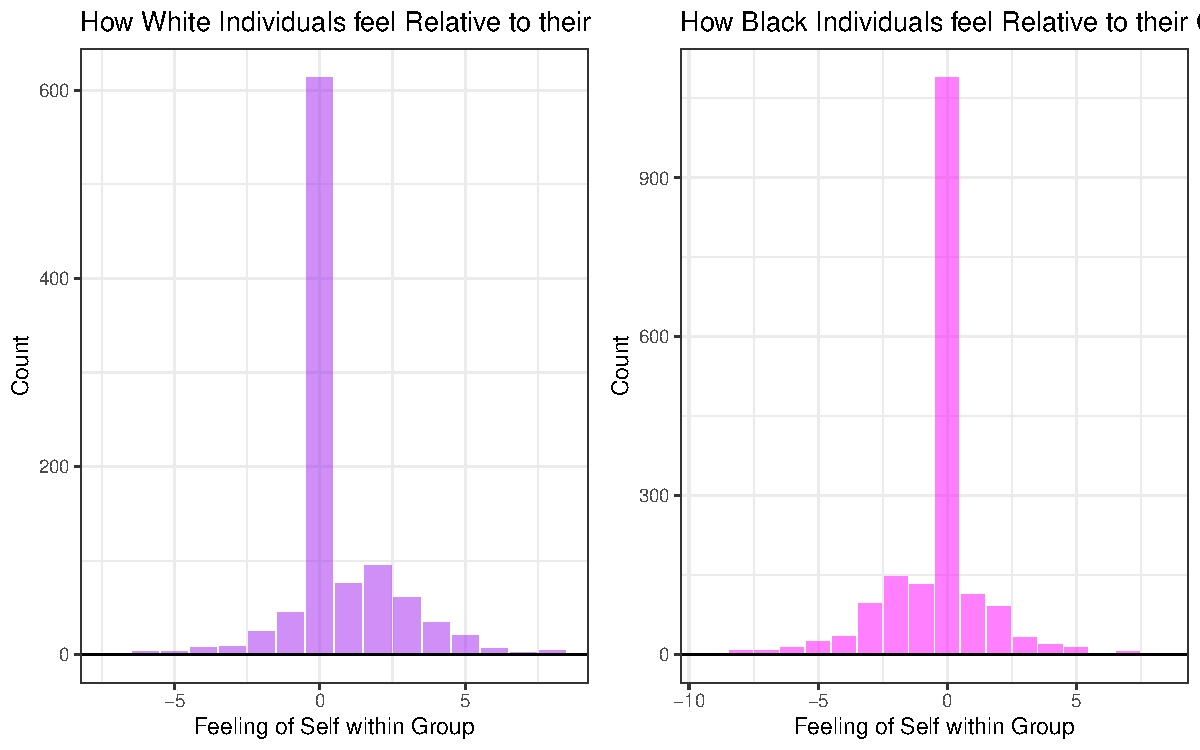
\includegraphics{HW1-011}
\newline\centering{Figures 1 and 2: How Individuals Perceive Themselves Relative to their Group by Race}
\newline
\newline{Ladder Difference in this data set is defined as the difference between an individual's perceived status of their group and the same individual's perceived status of themselves as an individual. By finding the difference between these two values, we are able to gauge how an individual feels relative to their group. 
While the predominant individual perception is that the individual perceives themselves to be an average member of their own group, there is slight variation between white and black individuals. White individuals in the sample have more observations that are positive than negative, meaning that white individuals perceive themselves more often to be lower on the social ladder compared to their group. Black individuals in the sample, however, have more negative observations relative to white individuals. This shows that black individuals more often view themselves as being better than their social group.}
\newpage
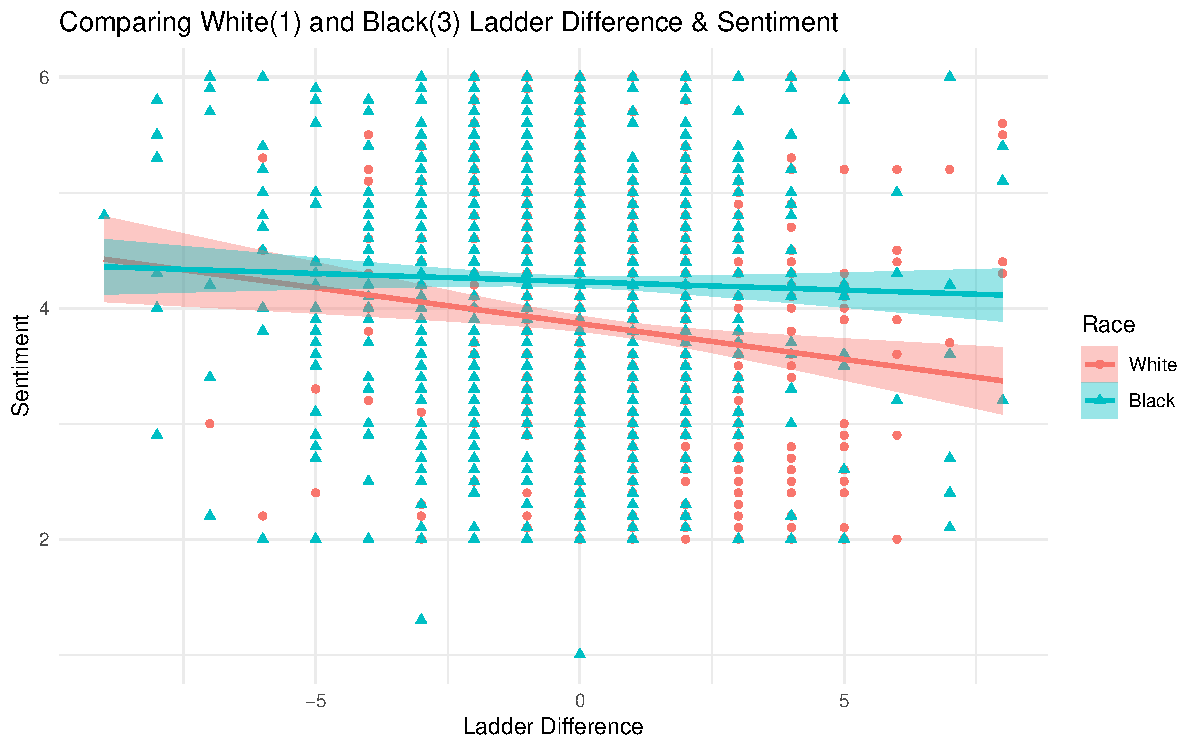
\includegraphics{HW1-012}
\newline\centering{Figure 3: Difference in General Sentiment by Difference in Perceived Individual and Group Status and Race}
\newline
\newline{This graph compares the Black and White sample in their individual sentiments and their Ladder Differences. As stated before, Ladder Difference is how individuals gauge themselves relative to their group, with positive values indicating individuals perceive themselves to be lower on the social ladder relative to their group and the opposite for negative values. Sentiment can be seen as an individual's emotions when taking the survey. Greater values indicate more positive emotions. As we can see from the graph, white individuals have a downward trend, indicating that positive emotions while taking the survey are correlated with individuals perceiving themselves to be higher on the social ladder relative to their group. Black individuals have a horizontal trend, indicating that individual feelings were the same when taking the survey regardless of how a Black person perceived themselves relative to their group. It's also important to note that Black individuals, on average, had a higher sentiment score relative to their white peers for any ladder difference greater than -7.5. }
\newpage
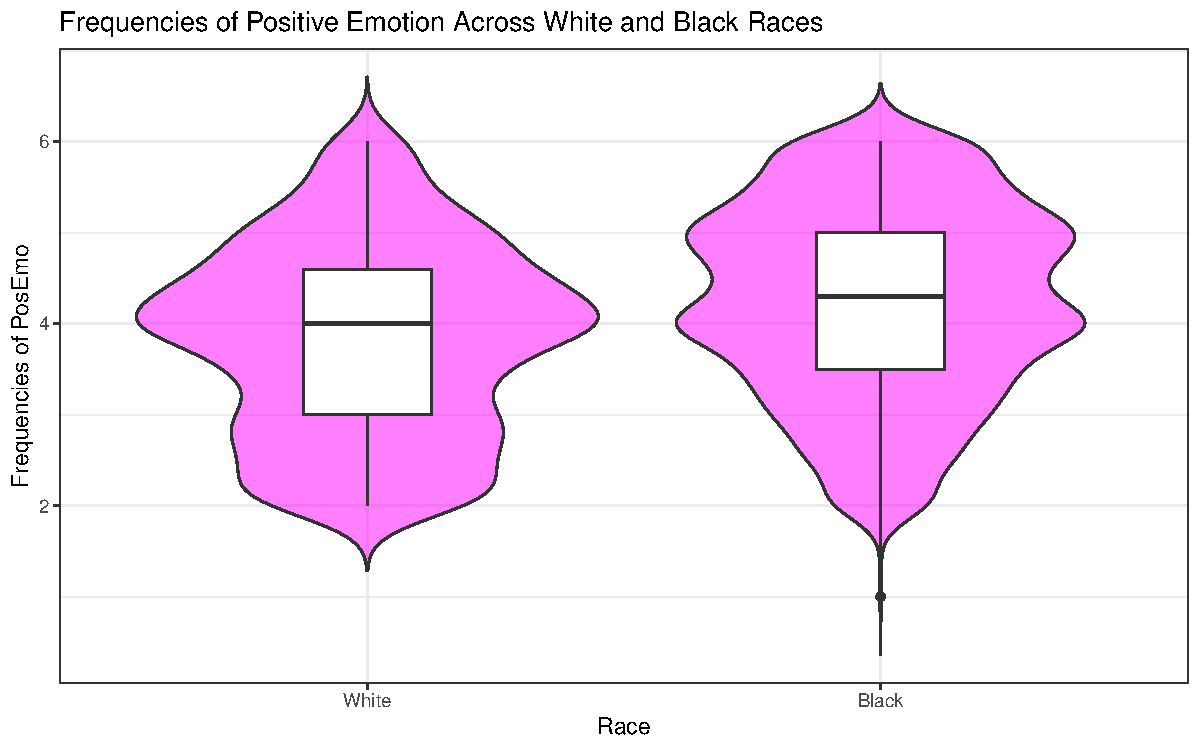
\includegraphics{HW1-013}
\newline\centering{Figure 4: Comparing Individual Sentiment Across Race}
\newline
\newline{This plot shows us the difference in distribution of positive emotions among white individuals and black individuals, respectively.We used a violin plot because positive emotion, in this case, is a continuous variable which is the average of many positive sentiment numerical metrics. The overlaid boxplots allows us to compare the 25th percentile, the median, and the 75th percentile easily between racial groups. As we can see, black individuals tend to feel more positive emotions, where a higher PosEmo value corresponds to more positive feelings, since the first quartile, median, and third quartile values are all higher. There is a slight left skew in the distribution of positive emotions for black individuals, with the median between two local peaks, and there is only one clear maximum for white individuals.}
\newpage
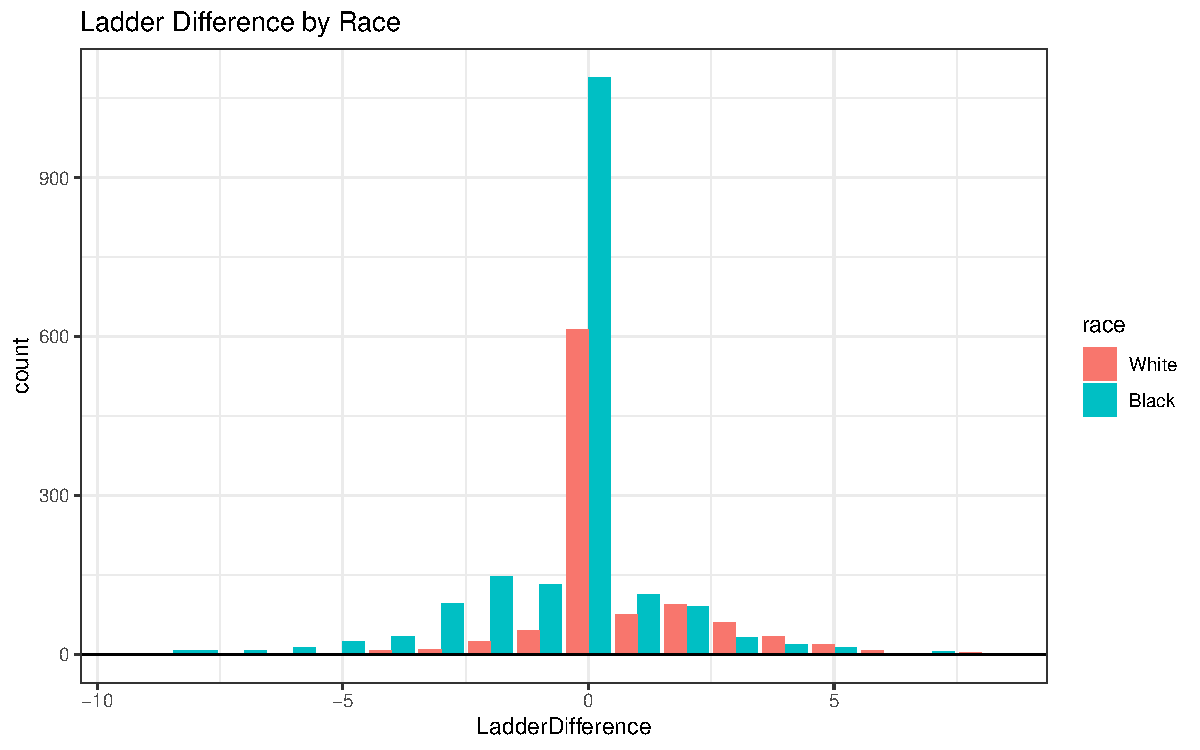
\includegraphics{HW1-014}
\newline\centering{Figure 5: Difference in Perceived Individual versus Group Status}
\newline
\newline{This plot shows us a side by side comparison of the Ladder Differences for two races: white, and black. Ladder difference, in this case, shows us how each individual feels they are perceived relative to their racial group. As we can see in the large blue bar at LD = 0, many black individuals tend to think of themselves as perceived in the same way as their group, thus yielding a difference of zero. A negative value, in this case, would indicate that the individual feels they are perceived better than their group; looking at values for LD that are less than zero, we see that black individuals tend to feel this way more than white individuals. Beyond LD = 0, which signfies that an individual feels they are perceived more poorly than their group, there is no obvious trend between black individuals and white individuals.}

\textbf{Other Attempts:}
\begin{Schunk}
\begin{Sinput}
> #sentiment of individual taking the survey
> ggdat<-data.frame(y=dat.wb1$PosEmo[which(dat.wb1$Race==1)]) #sentiment of white people
> p1<-ggplot(data=ggdat,aes(x='',y=y))+
+   geom_violin(fill="green",
+               #trim=FALSE,
+               alpha=0.5,
+               show.legend = FALSE) +
+   geom_boxplot(width=.25, fill="white") +
+   xlab('') +
+   ylab("Emotion Level") +
+   ggtitle("Sentiment of White Surveyors") +
+   theme_bw()
> ggdat<-data.frame(y=dat.wb1$PosEmo[which(dat.wb1$Race==3)]) #sentiment of black people
> p2<-ggplot(data=ggdat,aes(x='',y=y))+
+   geom_violin(fill="lightgreen",
+               #trim=FALSE,
+               alpha=0.5,
+               show.legend = FALSE) +
+   geom_boxplot(width=.25, fill="white") +
+   xlab('') +
+   ylab("Emotion Level") +
+   ggtitle("Sentiment of Black Surveyors") +
+   theme_bw()
> grid.arrange(p1,p2,ncol=2)
\end{Sinput}
\end{Schunk}

\begin{Schunk}
\begin{Sinput}
> #comparing white and black ladderdiff and posemo
> ggdat<-data.frame(x=dat.wb1$LadderDiff[which(dat.wb1$Race==1)], y=dat.wb1$PosEmo[which(dat.wb1$Race==1)]) #which specifies white
> t1<-ggplot(data=ggdat, aes(x=x,y=y)) +
+   geom_point(size=2,shape=18,color='violet') + #shape, size and color of points
+   geom_smooth(method = lm, fill="lightblue") + #adds regression line, confidence interval color
+   xlab("Ladder Difference") +
+   ylab("Sentiment") +
+   ggtitle("White Ladder Difference versus Individual Sentiment")
> ggdat<-data.frame(x=dat.wb1$LadderDiff[which(dat.wb1$Race==3)], y=dat.wb1$PosEmo[which(dat.wb1$Race==3)])
> t2<-ggplot(data=ggdat, aes(x=x,y=y)) +
+   geom_point(size=2,shape=18,color="purple") + #shape, size and color of points
+   geom_smooth(method = lm, fill="lightblue") + #adds regression line, CI color
+   xlab("Ladder Difference") +
+   ylab("Sentiment") +
+   ggtitle("Black Ladder Difference versus Individual Sentiment")
> grid.arrange(t1,t2,ncol=2)
\end{Sinput}
\end{Schunk}

\begin{Schunk}
\begin{Sinput}
> #what do ladderdiff and posemo mean
> #laddergroup - where would you place your group of people
> #ladderself - where would put yourself
> #posemo - how people feel when taking the survey
>   #relationship between how people feel when taking the survey
> 
> #what we got from office hours
> ggdat<-data.frame(x=dat.wb1$LadderDiff[which(dat.wb1$Race==3)])
> ggplot(data=ggdat, aes(x=x,y=..count..))+
+   geom_bar()
> ggdat<-data.frame(LD=dat.wb1$LadderDiff,race=dat.wb1$Race)
> ggplot(data=ggdat,aes(x=LD,fill=race))+
+   geom_bar(position=position_dodge()) #we unstacked
> ggdat<-data.frame(PE=dat.wb1$PosEmo,race=dat.wb1$Race)
> #failed attempt number 2 where I didn't know what data to extract
> ggdat<-data.frame((dat.wb1$LadderDiff))
> colnames(ggdat)=c("LadderDiff", "PosEmo")
> p1<-ggplot(data=ggdat, aes(x=LadderDiff)) +
+   geom_bar(stat = "identity",
+     color= "black",
+            fill= "lightblue") +
+   xlab("LadderDiff") +
+   ylab("Frequency") +
+   ggtitle("Frequency of LadderDiff for Black and White Surveyors") +
+   geom_hline(yintercept=0) +
+   theme_bw()
> p1
> 
> #ggdat2<-data.frame(PosEmo=dat.wb$PosEmo,race=dat.wb$Race)
> #ggplot(data=ggdat2,aes(x=PosEmo,fill=race))+
> #  geom_bar(position = position_dodge()) #don't leave it stacked- put side by side
> 
> #ggdat_white<-data.frame(table(data.frame(filter(dat.wb$LadderDiff, Race == 1))))
> #colnames(ggdat_white)=c("LadderDiff","PosEmo")
> #p_white<-ggplot(data=ggdat_white,aes(x=LadderDiff,y=PosEmo)) + #tell ggplot which data to use
> #  geom_bar(stat="identity",           #plot the count (no transformation needed)
> #           color="black",             #bar outline color
> #           fill="lightblue")        + #bar colors
> #  xlab("Ladder Difference")              + #x axis label
> #  ylab("Positive Emotion")                 + #y axis label
> #  ggtitle("Positive Emotion vs Ladder Difference") + #add title to plot
> #  geom_hline(yintercept=0)          + #adds a line for the x-axis
> #  theme_bw()                     #removes grey background
> #p_white
> 
> # tried to plot all of the information in one graph
> # not the prettiest way to do that
> # colnames(ggdat)=c("LadderDiff", "PosEmo")
> # p1<-ggplot(ggdat, aes(x=LadderDiff)) +
> #   #  geom_histogram(bins=10, #how many bins to use
> #   #                 fill = "lightblue",
> #   #                 color="black") +
> #   geom_bar()+
> #   xlab("Difference between the Group and Individual") +
> #   ylab("Emotion") +
> #   ggtitle("Emotions with respect to Ladder Difference") +
> #   theme_bw() +
> #   geom_hline(yintercept=0)
> # p1
\end{Sinput}
\end{Schunk}
\newpage


\item \textbf{(Data Cleaning and Summary)} Recreate the supplementary materials posted under 
this homework on Moodle. You can omit the statistical tests until we get there. 
\begin{Schunk}
\begin{Sinput}
> dat.comparison<-read.csv("https://cipolli.com/students/data/comparisonData.txt",
+                          header=T,sep=",")
\end{Sinput}
\end{Schunk}
\item \textbf{(Probability I)} The zinc-phosphate coating on the threads of steel tubes used in oil and gas wells is critical to their performance. However, 12 percent of all tubes receive an improper amount of coating (either much too low or much too high). That is, about 12 percent of the tubes are defective.
Assume that the tubes are independent. 
\begin{enumerate}
  \item If we take a sample of 10 tubes, what is the probability at least 2 are defective?
  \item If we continually observe tubes until we find the first defective tube, what is the 
  probability we will observe no more than 3 tubes?
  \item If we continually observe tubes until we find the second defective tube, what is the
  probability we will observe more than 4 tubes?
\end{enumerate}

\textbf{(Probability II)}Sowbugs are primarily nocturnal, thrive in a moist environment, and they eat decaying leaf
litter and vegetable matter. Suppose that Y , the number of sowbugs on a square-foot plot,
follows a Poisson distribution with $\lambda = 15.$
\begin{enumerate}
  \item Find the probability that a square-foot plot contains exactly 10 sowbugs.
  \item In terms of the Poisson PMF, write an expression for $P(Y >= 100)$.
\end{enumerate}

\textbf{(Probability III)} Explore all the plots for continuous data to compare the 
two vectors of data \texttt{x1} and \texttt{x2} loaded using the code above. Reflect on 
the importance of creating several graphs. Compare the likelihood of each data vector
being from the Gaussian($\mu=0$,$\sigma=1$) distribution and compare this to your
visual interpretation.
\begin{Schunk}
\begin{Sinput}
> dat.x<-read.csv("https://cipolli.com/students/data/HW1-twoDatasets.txt",
+                 header=T,sep=",")
\end{Sinput}
\end{Schunk}

\newpage
\item \textbf{Estimation} Consider  data originally from a study of the nesting horseshoe crabs \citep{brockmann1996satellite}. Each female crab in the study had a male crab attached to her in her nest. The study investigated factors that affect whether the female crab had any other males, called satellites, residing nearby her. Explanatory variables thought possibly to affect this included the female crab's color, spine condition, weight, and carapace width. The response outcome for each female crab is her number of satellites.
	 The sample is
	\begin{center}
		\begin{tabular}{|ccccccccccccccccc|}\hline
		 Number of Satellites& 0 & 1&  2&  3&  4&  5&  6&  7&  8&  9& 10& 11& 12& 13 &14& 15\\ \hline
		 Number of Observations&62& 16&  9& 19& 19& 15& 13&  4&  6&  3&  3&  1&  1&  1&  1&1\\\hline
 		\end{tabular}
	\end{center}
 	It is believed that the distribution of the number of satellites for a female crab is distributed Poisson$(\lambda)$ where the parameter $\lambda$ is of interest.
	\begin{enumerate}
	\item Calculate the method of moments estimator for $\lambda$.
	\item Find the maximum likelihood estimator for $\lambda$.
	\item Plot the data with the Poisson distribution fit with the MLE estimates. 
	How well does the distribution fit the data?
	\item Let's try another distribution - the zero-inflated Poisson distribution. Now, 
	it is believed that the distribution of the number of satellites for a female crab is
	distributed Poisson$_0(\lambda,\sigma)$ where the parameters $\lambda$ and $\sigma$ 
	are of interest. Find the method of moments estimators for both $\sigma$ and $\lambda$.
	 \[f_X(x|\lambda,\sigma)=(1-\sigma)\frac{\lambda^x e^{-\lambda}}{x!}I(x\geq1) + (\sigma+(1-\sigma)e^{-\lambda}) I(x=0)\]
	 \item Find the maximum likelihood estimator for $\lambda$ and $\sigma$.
	\item Plot a histogram of the data with the zero-inflated Poisson distribution fit with the MLE estimates. How well does the distribution fit the data?
	\end{enumerate}
\textbf{Solution:}
\textbf{Setting Up the Data:}
\begin{Schunk}
\begin{Sinput}
> #formatting the data in different ways
> numofsatellites <- c(0:15)
> numofobs <- c(62, 16, 9, 19, 19, 15, 13, 4, 6, 3, 3, 1, 1, 1, 1, 1)
> crabby_data1 <- data.frame(numofobs,numofsatellites)
> #create a vector of crab data
> crabby_data <- c(rep(0, 62),
+                  rep(1,16),
+                  rep(2, 9),
+                  rep(3, 19),
+                  rep(4, 19),
+                  rep(5,15),
+                  rep(6, 13),
+                  rep(7, 4),
+                  rep(8, 6),
+                  rep(9, 3),
+                  rep(10,3),
+                  rep(11, 1),
+                  rep(12, 1),
+                  rep(13, 1),
+                  rep(14, 1),
+                  rep(15, 1))
> #Other Attempts
> #sumofobs <- sum(numofobs)
> #sample_mean=sum(numofobs * numofsatellites)/sumofobs
\end{Sinput}
\end{Schunk}

\textbf{Part A:}
\begin{Schunk}
\begin{Sinput}
> #install.packages("gmm") #install packages
> library(gmm) #load packages
> set.seed(69) #makes data comparable to others
> g<- function(x,theta) { #(data, theta)
+   #set the sample and population moments to be equal
+   b <- theta
+   m1 <- b - mean(x) #moment
+   return(m1)
+ }
> gmm(g=g,#function
+     x=crabby_data,#data
+     t0=mean(crabby_data), #inital guess
+     method="Brent",#univariate
+     lower=0, #reasonable lower
+     upper=1.5*max(crabby_data)) #reasonable upper
\end{Sinput}
\begin{Soutput}
Method
 twoStep 

Objective function value:  3.983414e-30 

Theta[1]  
   2.977  

Convergence code =  0 
\end{Soutput}
\end{Schunk}

\textbf{Part B:}
\begin{Schunk}
\begin{Sinput}
> #Part B - find maximum likelihood estimator for lambda
> LL <- function(lambda) { #function inputting lambda
+   return(-1*sum(dpois(crabby_data, lambda = lambda, log = TRUE))) #likelihood of distribution
+ }
> a <- optim(fn = LL, #function
+       par=mean(crabby_data), #best guess
+       method="Brent", #
+       lower=0, 
+       upper=1.5*max(crabby_data))
> a
\end{Sinput}
\begin{Soutput}
$par
[1] 2.977011

$value
[1] 505.4901

$counts
function gradient 
      NA       NA 

$convergence
[1] 0

$message
NULL
\end{Soutput}
\end{Schunk}

\textbf{Part C:}
\begin{Schunk}
\begin{Sinput}
> library(ggplot2) #load library
> crabby_data1 <- tibble(crabby_data) #reformatting for histogram
\end{Sinput}
\end{Schunk}

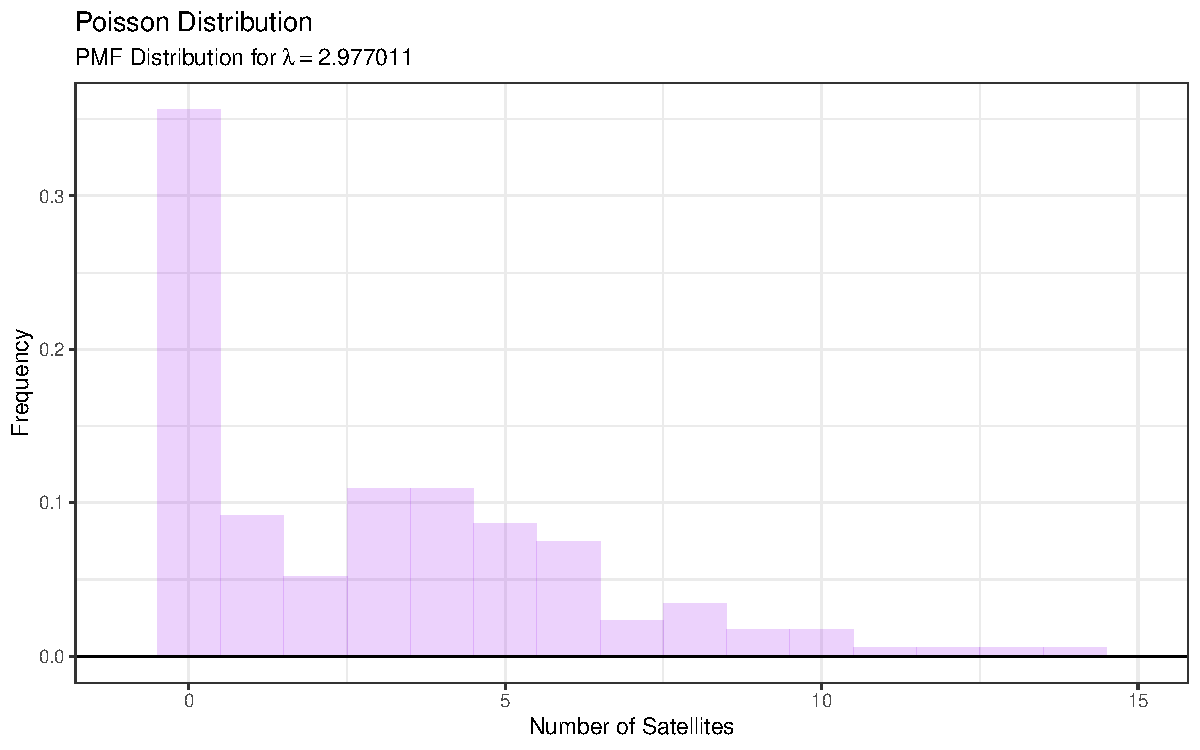
\includegraphics{HW1-024}
\newline
\centering{Figure: The Poisson Distribution fit with MLE Estimation}
\newline
This plot shows the PMF of a discrete random variable X, given by bquote (f[x] (x)) = P(X=x) for all x. In the context of this problem, the discrete random variable X is the number of satellites found around the observed female horseshoe crabs. Assuming our observations have an underlying Poisson distribution, which is used to represent the number of times a specific event (where an event is an observation of X satellites around a female horseshoe crab) occurs in a given time or space, we are able to obtain a Maximum Likelihood Estimate for lambda, the parameter of the model. The MLE maximizes the likelihood of having a specific value for lambda given the underlying Poisson distribution (i.e. Given the distribution, the likelihood of its true lambda value being 1,000,000 is essentially zero, whereas having a lambda value near the sample mean, is likely the most probable because the sample mean is usually a good indicator of the theoretical mean); in our case, the MLE gives us 2.98, which we then use in the below graph of the PMF of our Poisson distribution. As we can see, the Poisson distribution fit with the MLE estimate fits the data well, and we can see this because the lambda values are most likely between 2 and 4, which is also observable in the data given to us. When we compare the MLE estimate for lambda fits the data much better than the MoM estimate for lambda. It is important to note that while the distribution fits the data well, it does not properly account for the number of zero observations in our dataset. 

\textbf{Part D:}
\begin{Schunk}
\begin{Sinput}
> #Part D - zero-inflated poisson distribution
> set.seed(69)
> g_1<- function(x,theta) { #(data, theta)
+   #set the sample and population moments equal
+   lambda = theta[1] 
+   sigma = theta[2]
+   EX = (1-sigma)*lambda
+   varX = (1-sigma) * (lambda + lambda^2) - ((1-sigma)*lambda)^2
+   m1 <- EX - x
+   m2 <- varX - (x-EX)^2
+   return(c(m1, m2)) #return moments
+ }
> gmm(t0= c(0,60), #best guess
+     g=g_1,#function
+     x=crabby_data) #data
\end{Sinput}
\begin{Soutput}
Method
 twoStep 

Objective function value:  0.4674955 

 Theta[1]   Theta[2]  
 0.049805  -0.246094  

Convergence code =  0 
\end{Soutput}
\end{Schunk}

\textbf{Part E:}
\begin{Schunk}
\begin{Sinput}
> #Part E - find the maximum likelihood estimator for lambda and sigma
> alexa <-function(x, lambda, sigma) { #function given, probability of x given lambda and sigma
+   log(((1-sigma)*(((lambda^x)*(exp(-lambda))/(factorial(x))))*(x>=1)) + ((sigma + (1 - sigma)*(exp(-lambda)))*(x==0)))
+ }
> LL1 <- function(x, theta, neg=FALSE) {#takes the data and theta
+   sigma<-theta[1]
+   lambda<-theta[2]
+   #applies a function to a vector and sums the values
+   ll <-sum(sapply(X=crabby_data, FUN = alexa, sigma = sigma, lambda = lambda))
+   ifelse(!neg,ll,-ll)
+ }
> c <- optim(fn = LL1, #function
+            x = crabby_data, #data
+            par=c(min(crabby_data),max(crabby_data)), #best guess
+            neg=TRUE)
> c
\end{Sinput}
\begin{Soutput}
$par
[1] 0.3494643 4.5775109

$value
[1] 389.4734

$counts
function gradient 
      63       NA 

$convergence
[1] 0

$message
NULL
\end{Soutput}
\end{Schunk}

\textbf{Part F:}
\begin{Schunk}
\begin{Sinput}
> #Part F - plot a histogram of zero-inflated poisson distribution fit
> 
> library(ggplot2)
> alexa_non_log <-function(x, lambda, sigma) { #nonlog function to use for plotting
+   (((1-sigma)*(((lambda^x)*(exp(-lambda))/(factorial(x))))*(x>=1)) + ((sigma + (1 - sigma)*(exp(-lambda)))*(x==0)))
+ }
> #creating a distribution using sigma and lambda
> zero_pois_dis <- sapply(X=0:15, FUN = alexa_non_log, sigma=0.3494643, lambda=4.5775109)
> test1 <- data.frame(x=c(0:15), dist = zero_pois_dis)
> #install.packages("tidyverse") #install tidyvevrse
> library(tidyverse) #load tidyverse
> crabby_data1 <- tibble(crabby_data) #reformatting for histogram
> #ggdat <- data.frame(x=c, f1=zero_pois_dis)
\end{Sinput}
\end{Schunk}

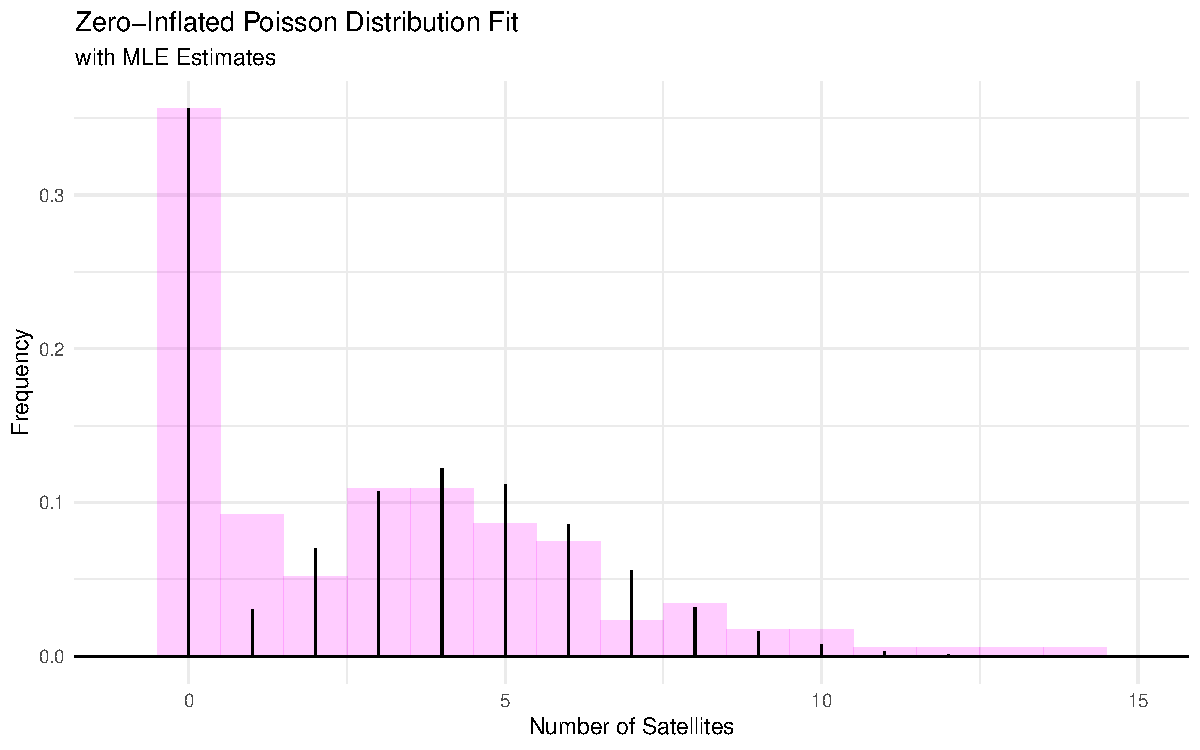
\includegraphics{HW1-028}
\newline
\centering{Figure: The Zero-Inflated Poisson Distribution}
\newline
As we can see, the Zero-Inflated Poisson Distribution actually fits better than the Poisson Distribution because the Poisson Distribution did not fit to the large number of zero values. However, we can see in this plot that the Zero-Inflated Poisson Distribution almost perfectly accounts for the amount of zeros we have in our data set. In fact, it is almost the same distribution as the Poisson Distribution besides the fact that it also accounts for the zero observations. 
	\end{enumerate}
\bibliography{bib}
\end{document}
